\documentclass{article}
\usepackage{graphicx} % Required for inserting images
\usepackage{geometry}
\usepackage{circuitikz}
\usepackage{siunitx}
\usepackage{CJKutf8}
\usepackage{amsmath}
\usepackage{amssymb}
\usepackage{caption}
\usepackage{float}
\usepackage{subcaption}
\geometry{top=5mm, left=30mm, a4paper}

\title{Antoniou Inductance-Simulation Circuit Prelab}
\author{梁程捷 (B11901136), 吳奕娃 (B11901080)}
\date{}


\begin{document}
\begin{CJK*}{UTF8}{bkai}

\maketitle

\section*{Antoniou Inductance-Simulation Circuit}
Use two 741 Op-Amps to construct the circuit in Figure (c), and follow the steps below: \\
1. Record the output($V_o$) waveform for $R_5$ = 10\unit{\kilo\ohm}. \\
2. Record the output($V_o$) waveform for $R_5$ = 1.1\unit{\kilo\ohm}. \\
3. Record the output($V_o$) waveform for $R_5$ = 400\unit{\ohm}. \\
4. Record the output($V_o$) waveform for $R_5$ = 200\unit{\ohm}. \vspace{3mm}\\
\textbf{Voltage source: } $V_{i,pp} = 1$ \unit{\volt} (f = 1\unit{\kilo\hertz}) \\
\textbf{Resistors: }$R_1$ = $R_3$ = 510\unit{\ohm}, $R_2$ = 100\unit{\ohm} \\
\textbf{Capacitors: }$C_4$ = 0.01\unit{\micro\farad}, $C_6$ = 0.1\unit{\micro\farad} \\

\begin{figure}[h]
    \begin{center}
        \begin{subfigure}[b]{0.4\textwidth}
            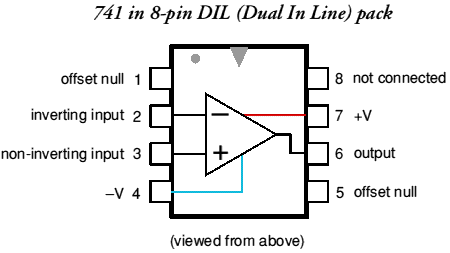
\includegraphics[width=\textwidth]{741Pinout.png}
            \caption*{Figure (a): 741 Op-Amp Pinout}
        \end{subfigure}
        ~
        \begin{subfigure}[b]{0.4\textwidth}
            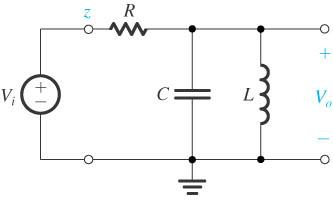
\includegraphics[width=\textwidth]{BP.png}
            \caption*{Figure (b): RLC band-pass filter}
        \end{subfigure}
    \end{center}
\end{figure}

\begin{figure}[h]
    \begin{center}
        \begin{subfigure}[b]{0.6\textwidth}
            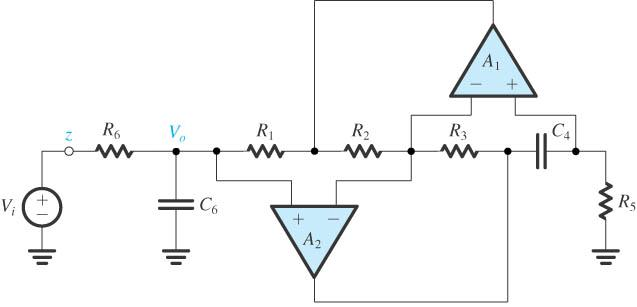
\includegraphics[width=\textwidth]{BP_Antoniou_Inductance.png}
            \caption*{Figure (c): RLC band-pass filter using Antoniou Inductance}
        \end{subfigure}
    \end{center}
\end{figure}


\end{CJK*}
\end{document}